\documentclass[a4paper, 11pt]{article}
\usepackage{amsmath}
\usepackage{amssymb}
\usepackage{fancyhdr}
\usepackage{graphicx}
\usepackage[english]{babel}
\usepackage[utf8x]{inputenc}
\usepackage[T1]{fontenc}
\usepackage{scribe}
\usepackage{listings}
\usepackage{algorithm}
\Scribe{Kriangsak Thuiprakhon}
\Lecturer{Kanat Tangwongsan}
\setlength{\headheight}{35pt}
\LectureNumber{8}
\usepackage{tikz}
\tikzset{every picture/.style={line width=0.75pt}} %set default line width to 0.75pt        
\LectureDate{DATE}
\LectureTitle{Application of Scan}
\lstset{style=mystyle}

\usepackage[margin=1in]{geometry}

\newcommand{\question}[2] {\vspace{.25in} \hrule\vspace{0.5em}
\noindent{\bf #1: #2} \vspace{0.5em}
\hrule \vspace{.10in}}
\renewcommand{\part}[1] {\vspace{.10in} {\bf (#1)}}

\newcommand{\myname}{Kriangsak Thuiprakhon: 6080163}
\newcommand{\myemail}{kriangsak.thi@student.mahidol.edu}
\newcommand{\myhwnum}{}

\setlength{\parindent}{0pt}
\setlength{\parskip}{5pt plus 1pt}
 
\pagestyle{fancyplain}
\lhead{\fancyplain{}{\textbf{FINAL EXAM}}}      % Note the different brackets!
\rhead{\fancyplain{}{\myname\\ \myemail}}
\chead{\fancyplain{}{ICCS240 }}

\begin{document}

\medskip                        % Skip a "medium" amount of space
                                % (latex determines what medium is)
                                % Also try: \bigskip, \littleskip

\thispagestyle{plain}
\begin{center}                  % Center the following lines
{\Large ICCS240: FINAL EXAM \myhwnum} \\
\myname \\
\myemail \\
\end{center}
\section{Multiple Choices}
\begin{enumerate}
\item False
\item False
\item True
\item True
\item False
\item True
\item True
\item False
\item False
\item True
\item False
\item False
\item True
\item False
\item True
\item False
\item True
\item True
\item False
\item True
\end{enumerate}
\section{SQL and Relational Algebra}
\begin{enumerate}
\item Given a database schemata:Product(pid,price),Order(oid,customer,pid,quantity). Write in SQL to find a list all products along with its total ordered quantities in descending
order of the amount.

\textsc{SQL:} 
\begin{verbatim}
 SELECT pid, sum(quantity) AS sum  FROM orders 
 GROUP BY pid  ORDER BY sum DESC;
\end{verbatim}
\item Write the following relational algebra expression in SQL, for relation R(a,b,c) and S(a,b,c):  $\pi _{a,b}(\delta_{a<0}(R))- \pi_{a,b}(S)$

\textsc{SQL:} 
\begin{verbatim}
 SELECT a.,b FROM R WHERE R.a <0 AND NOT EXISTS (SELECT a,b FROM S);
\end{verbatim}
\item SELECT a, d FROM R, S WHERE R.a > 240 and R.b = S.c.
\textsc{Relational Algebra:} $$\Pi_{a,d} (\delta_{a>240}(R) \bowtie_{b=c} (S))$$
\end{enumerate}
\section{Design Theory}
\begin{enumerate}
\item Given relation $R(A, B, C, D, E, G)$ and the set of functional dependencies $\mathcal{F}: A \rightarrow CD, AB \rightarrow DE, AD \rightarrow  G, BD \rightarrow E, D \rightarrow EG, E \rightarrow G$
Find a minimal basis of F.

\textsc{answer : }
\begin{itemize}
\item[1] Rewrite the FD into those with only one attribute on RHS. We obtain: 
\begin{align*}
A &\rightarrow C\\
A &\rightarrow D\\
AB &\rightarrow D\\
A D&\rightarrow G\\
BD &\rightarrow E\\
 D &\rightarrow E\\
 D &\rightarrow G\\
 E &\rightarrow G\\
AB &\rightarrow B\\
\end{align*}

\item[2]  Remove trivial FDs (those where the RHS is also in the LHS). We obtain: In this casem noting can be removed
\item[3] Minimize LHS of each FD. We obtain: 
 \begin{align*}
A &\rightarrow C\\
A &\rightarrow D\\
A &\rightarrow D\\
D&\rightarrow G\\
D &\rightarrow E\\
 D &\rightarrow E\\
 D &\rightarrow G\\
 E &\rightarrow G\\
A &\rightarrow B\\
\end{align*}
\item[4]  Remove redundant FDs (those that are implied by others). We obtain: 
\begin{align*}
A &\rightarrow C\\
D &\rightarrow E\\
 E &\rightarrow G\\
A &\rightarrow A\\
\end{align*}
\end{itemize} 
\item Assume a relation R(A,B) has no NULL values. Write a SQL query that can check whether a functional dependency A ! B holds in R. Briefly explain why your query works.

\textsc{answer : }

\begin{verbatim}
SELECT * FROM R r1, R r2 WHERE r1.A=r2.A AND r1.B <> r2.B;
\end{verbatim} 
This query should return an empty table if A —> B holds. 
Why does this work? This is because:
(first, select A   iff $ r1.A=r2.A$ from the cross product)—AND— (second, B iff $r1.B <> r2.B$)
this means that for every  A in R, it is mapped strictly one-to-one to B in R.
This is why the resulting table is empty if $A \rightarrow B $holds.
\item Consider a relational R(A,B,C) having a functional dependency A ! B. If C is a candidate key for R, determine if R could be in BCNF (YES/NO). If YES, state the condition when/where R could be in BCNF. Otherwise, explain why R cannot be in BCNF.

\textsc{answer : }

No, because if C were to be a candidate key, FD A—> B has violated the condition to be in BCNF, that is ,every determinant has to be a candidate key. In this case, A is not a candidate key. Hence, R is not in BCNF

\end{enumerate}

\section{Storage and Indexing }
\begin{enumerate}
\item Consider a relationR(A,B) stored as a randomly ordered file. The only index on R is an \textit{unclustered} index on A. Suppose you want to retrieve all records where $A > 0$. Explain whether using the index is always the best alternatives. What about just simply performing file scanning instead of using the index?

\textsc{answer : }

Per the nature of query, we can see that it works in the way that it will filter every other elements that are 
at most zero. unclustered index is used to optimize filtering queries. One application of unclustered index is
filtered index. A filtered index is an optimized nonclustered index especially suited to cover 
queries that select from a well-defined subset of data. It uses a filter predicate to index a portion of rows in 
the table. A well-designed filtered index can improve query performance as well as reduce index 
maintenance and storage costs compared with full-table indexes.
The good thing about it is that creating a filtered index can reduce disk storage for nonclustered indexes 
when a full-table index is not necessary. You can replace a full-table nonclustered index with 
multiple filtered indexes without significantly increasing the storage requirements.
 
Performing a scan over A without indexing will result in a higher time compextity. 

\item Consider an application that required user to register their names. Assume at this moment the following users have registered their name in the following order (their age is in the parentheses):
$$alice(10), bob(20), carol(19), david(30), eve(15), frank(60), alex(10), chris(31), diana(99)$$
It is expected to have many more users in the future. The application tends to retrieve some
(sub) lists of users ordered by names, and sometimes ordered by their ages.
What index(es) should be built to help facilitate or improve the application query performance? Show how all of your proposed index(es) looks like. You must also specify any hash, comparison function or any related function you need to build your index(es).

\textsc{ANSWER} \\
To  improve upon performances, I propose clustered index on name attribute and \textit{unclustered} dynamic hashed-based index for the age attribute, specifically, a B+ tree. For the first part, I am using a clustered index so that it makes it easier to perform (sub) lists-of-users-ordered-by-names type of queries. With a B+ tree of degree k, this will be beneficial when querying for lists of users ordered by age. 

we can create a clustered index using: 
Assume that the application has database: $app(name varchar, age int)$.
\begin{verbatim}
CREATE UNIQUE CLUSTERED INDEX nameIndex ON app (name)
\end{verbatim}
If we use a B tree the result may look like this:

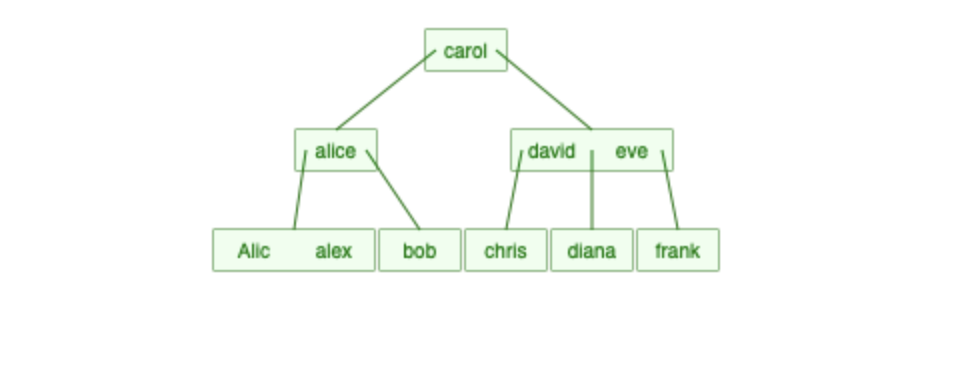
\includegraphics[width=\textwidth]{namesclustered.png}

This will index name records in an alphabetical order. 

for the age indexing, we can use a similar SQL query to create an index by:
\begin{verbatim}
CREATE UNIQUE INDEX idxAge ON app ( age ASC);
\end{verbatim}
This may result in a tree looking like the following:

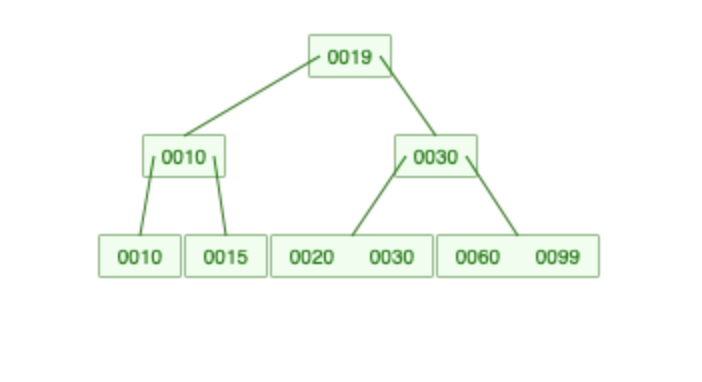
\includegraphics[width=\textwidth]{agetree.png}

\end{enumerate}
\section{Transaction and Concurrency Control}
\begin{enumerate}
\item Consider the actions R(X); W(X) taken by transaction T 1 on database object X. Give an example of another transaction T2 that, if run concurrently to T1 without some form of concurrency control, could interfere with T 1. Briefly explain why.

\textsc{answer}

$T_1: R(X); W(X)\\
T_2: W(X); R(X)\\
$
This causes an interference of in the case that the second transaction performs R(X) first and the first transaction has not yet written , T2 will abort. The value read by T1 would be invalid and the abort would be cascaded to T1 (according to some random website...).

\item Explain what it means for a schedule to avoid-cascading-aborts.

\textsc{answer}

A schedule is said to avoid cascading aborts if whenever a transaction reads an element, the transaction that has last written it has already committed. That is, cascadeless Schedule avoids cascading aborts/rollbacks (ACA) Schedules in which transactions 
read values only after all transactions whose changes they are going to read commit are called 
cascadeless schedules. Avoids that a single transaction abort leads to a series of transaction rollbacks. 
A strategy to prevent cascading aborts is to disallow a transaction from reading uncommitted changes 
from another transaction in the same schedule.\\
In other words, if some transaction $T_j$ wants to read value updated or written by some other 
transaction $T_i$, then the commit of $T_j $must read it after the commit of $T_i$.

\item
	\begin{itemize}
	\item[(i)] 
 Given a schedule:
                $$R2(C); R1(B); R1(A); W1(B); R3(A); W3(B); R3(C); W2(B)$$
Please answer the following questions.
Draw a precedence graph of the above schedule.

\textsc{answer}

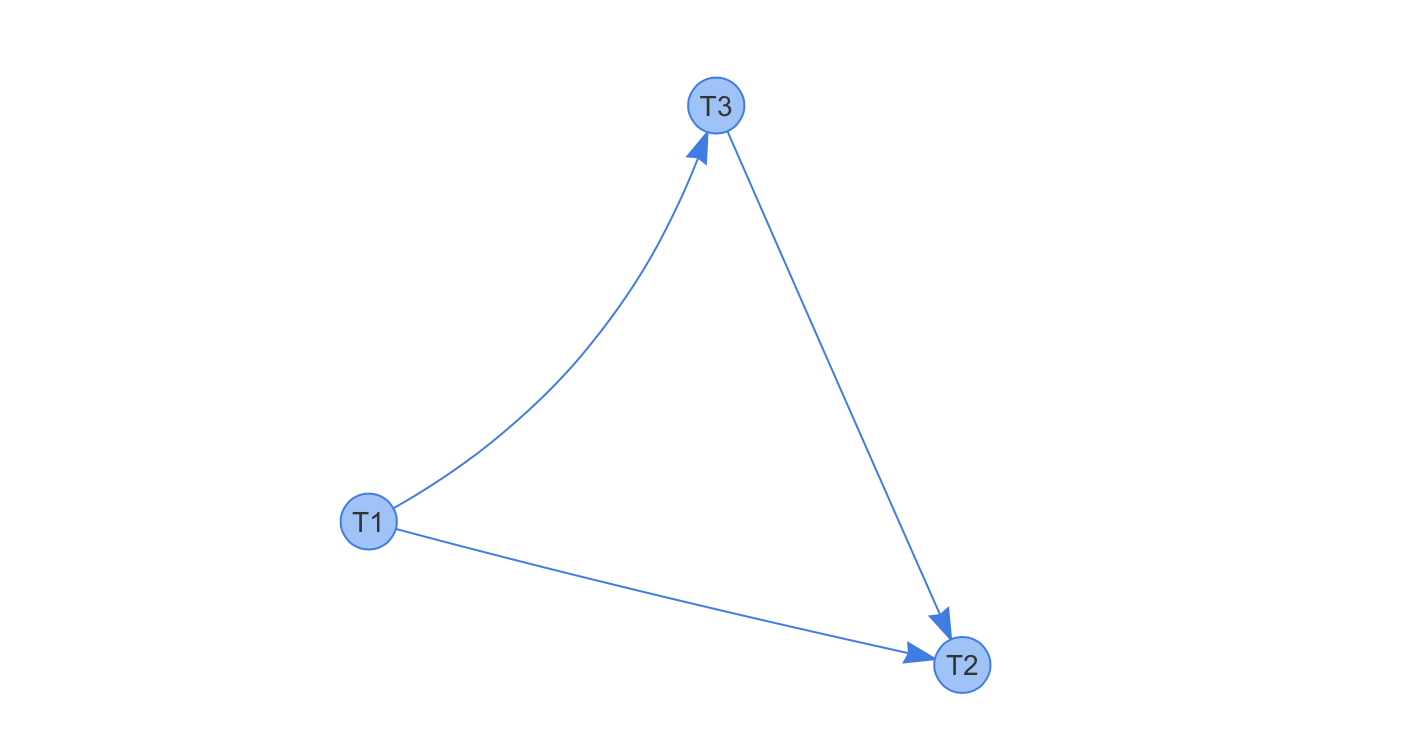
\includegraphics[width=\textwidth]{precedenceG.png}

	\item[(ii)] Is the schedule conflict serializable? If so, write YES and show the order in which the transaction would have to run in the equivalent serial schedule. Otherwise, write NO. (3pt)
	
	\textsc{answer}
	
	Since the graph is acyclic, the schedule is conflict serializable
	In Topological Sort, we first select the node with indegree 0, which is T1. This would be followed by T3 and T2. \\
	 Hence, the given schedule is conflict serializable since it is conflict equivalent to the serial schedule T1 T3 T2.
\end{itemize}	 
	\item No, only one transaction will lock A.
	Assume without loss of generality, take transaction, let's just take the first transaction for simplicity. From what we learned,  a  transaction is able to work on something of and only if other transactions stop before being able to lock B. now, the T1 can perform actions on B while locking it, then committing  to release A and B. This then causes no deadlocks.  
	\item i dont know
\end{enumerate}
\section{Query Execution and Optimization}
\begin{enumerate}
\item plans

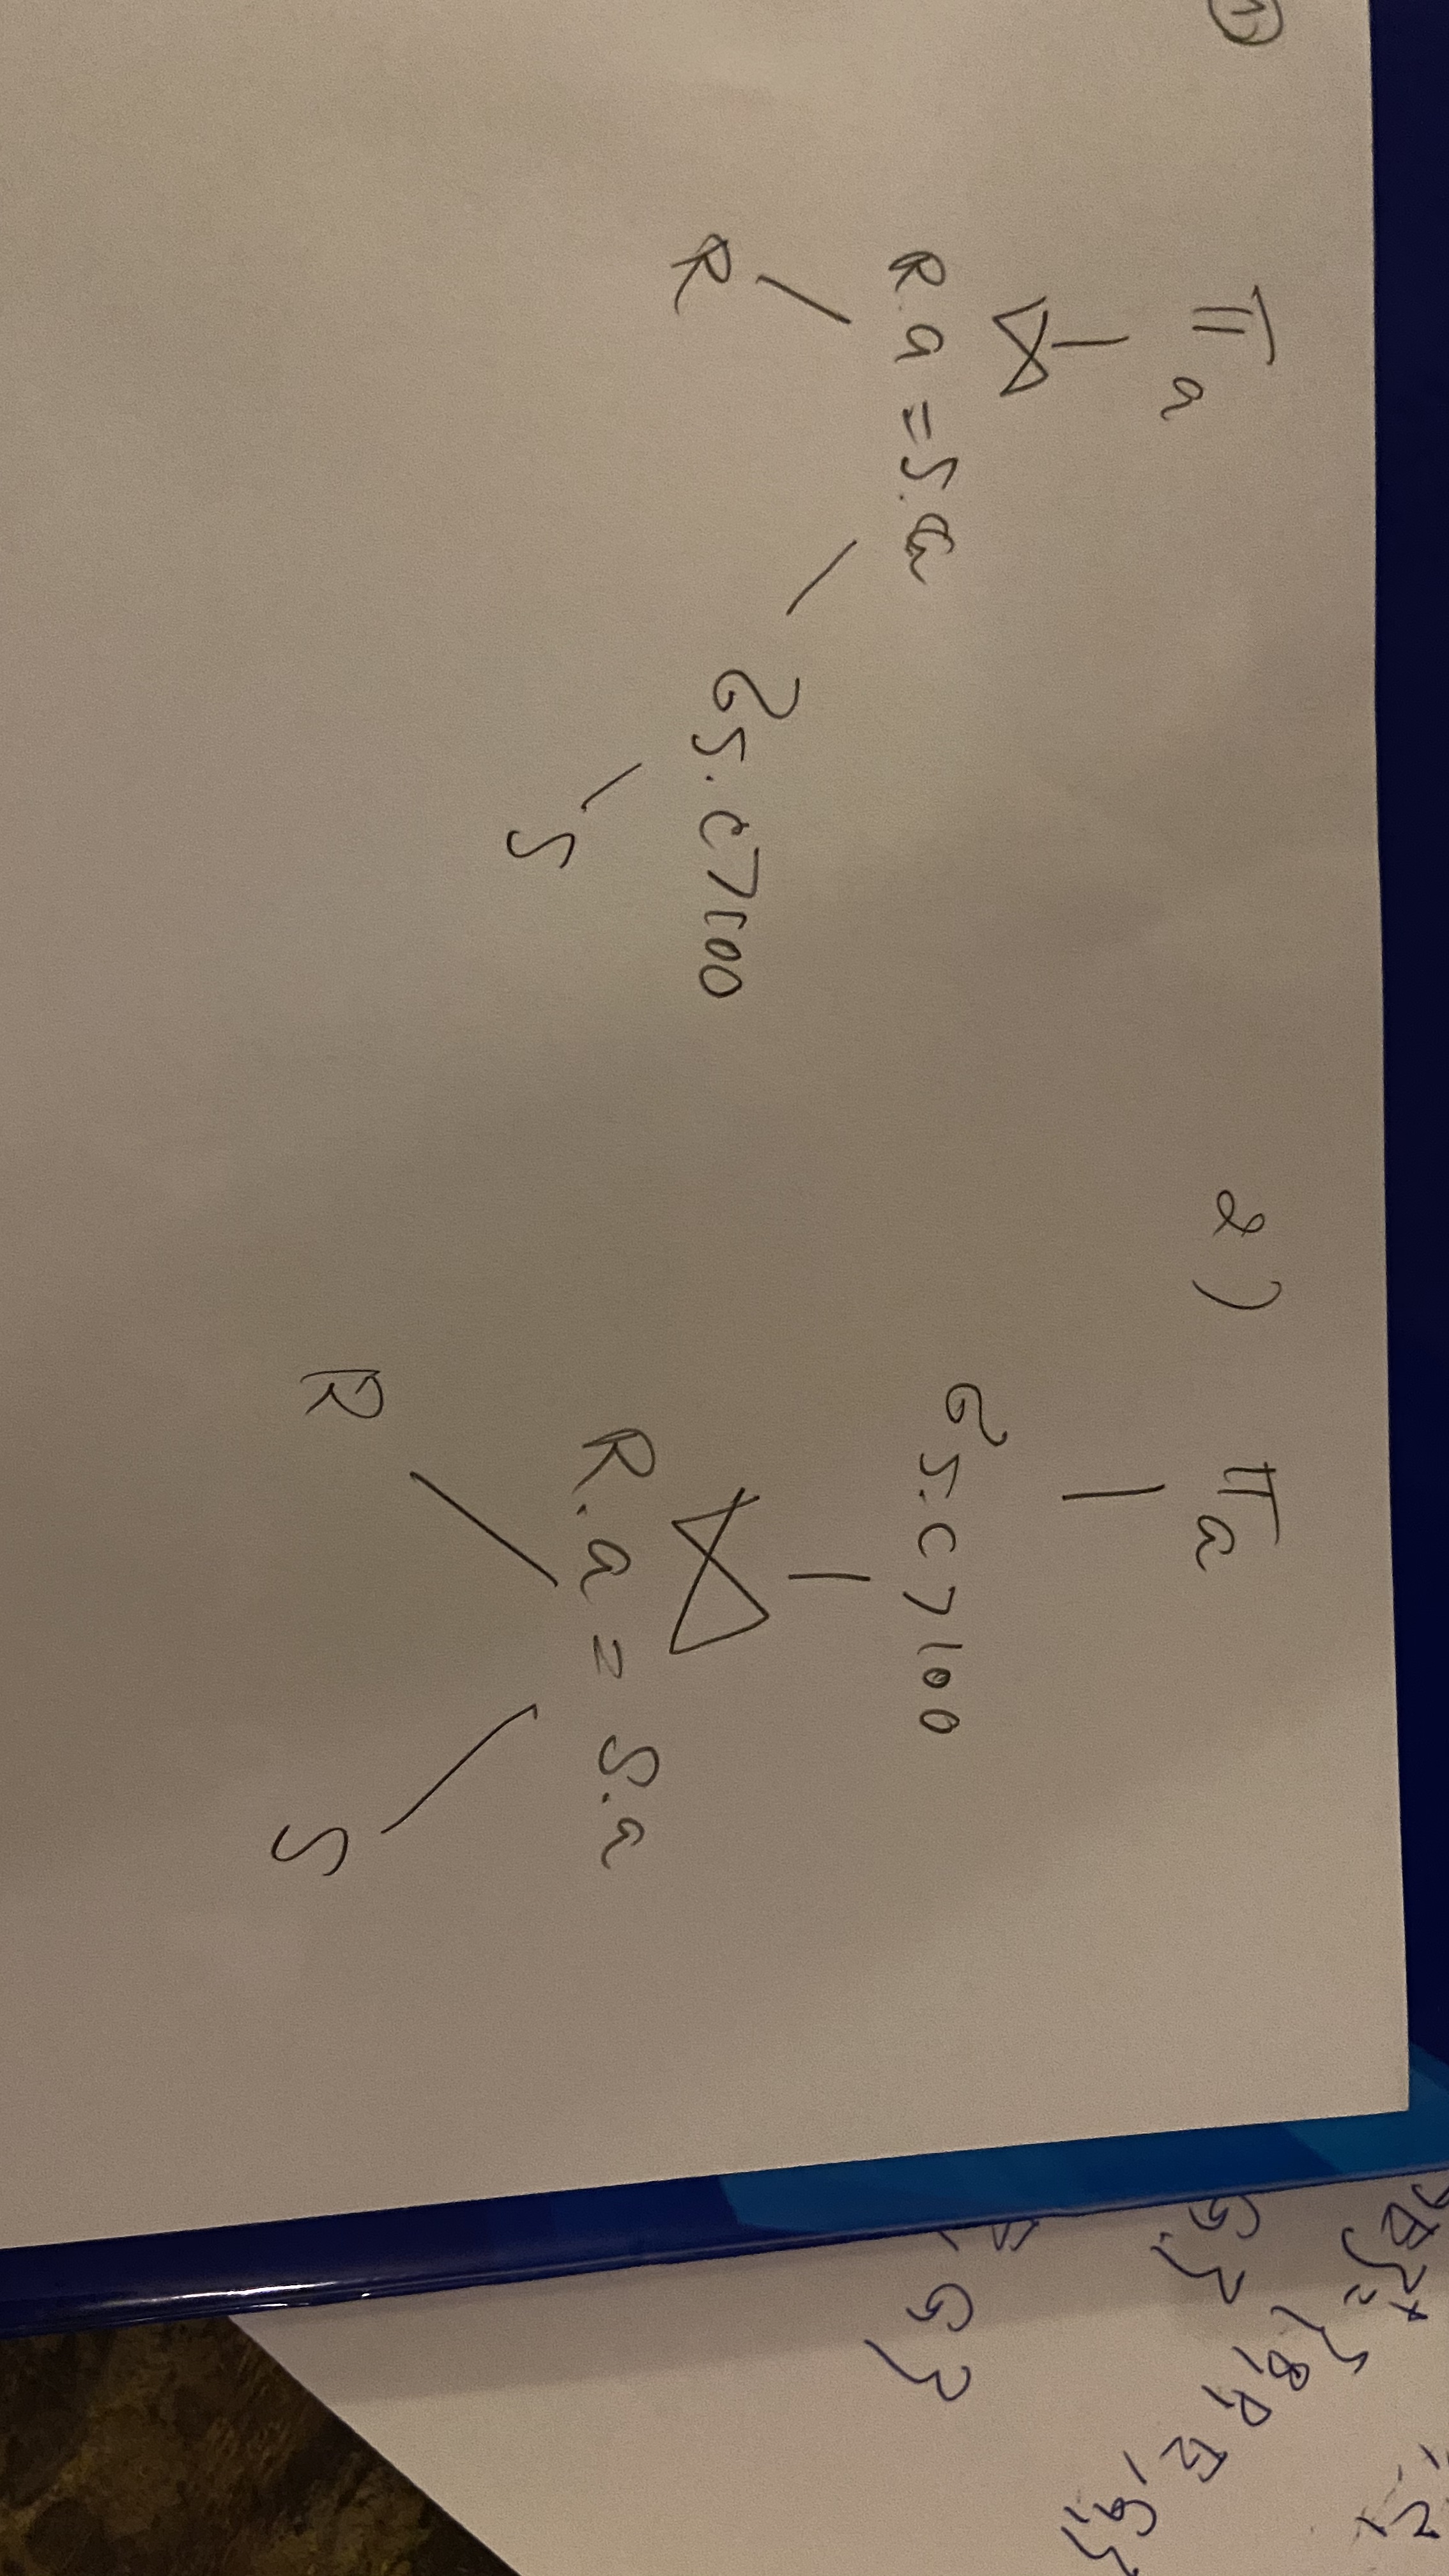
\includegraphics[width=\textwidth]{plans.jpg}

\item  I DON'T KNOW
\item
 a) B(R) = 10 I/O
b)  clustered: 10/10 = 1 ,  unclustered: 2000/10 = 200
c) assume LS,  B(R)+B(S)= 10 +80 = 90
d) B(R)= 10
e) 5B(R)+5B(S) = 50 + 400 = 450
f) 10 if no indexing 
g) $B(R) + 5(B(S) = 410$
h)$ B(R) + 5B(S)/90-B(R) =12$

\end{enumerate}


\section{Extra Credit}
\subsection{EXAM I}
\subsection{EXAM II}
\begin{itemize}
\item[4] 

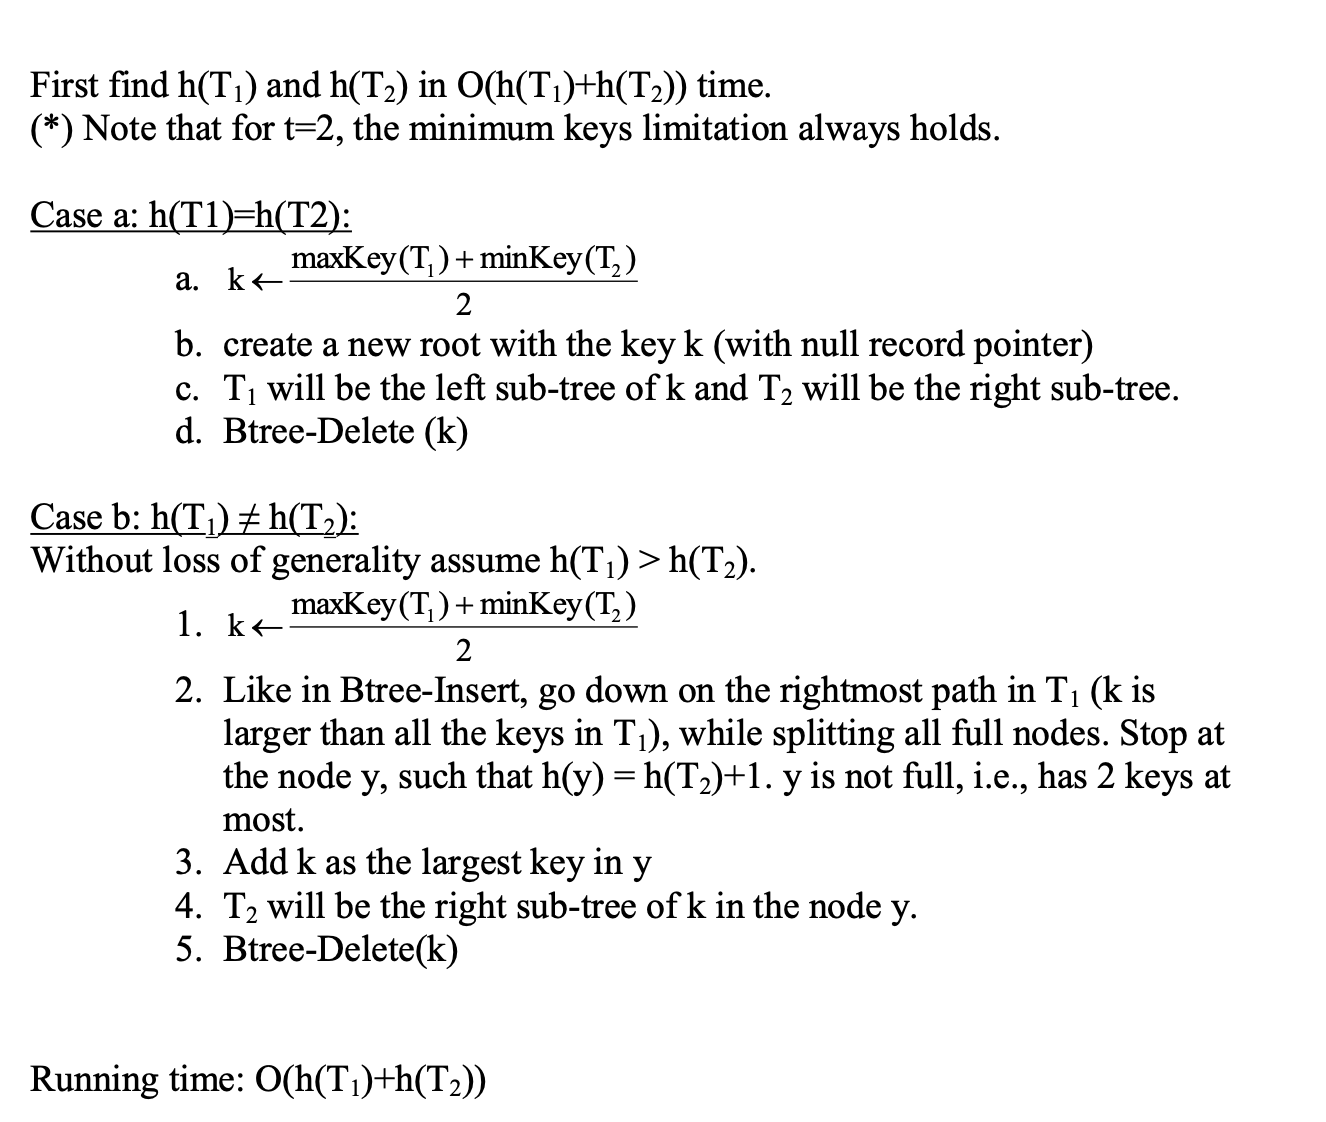
\includegraphics[width=\textwidth]{4.png}
\end{itemize}



\end{document}